% !TeX encoding=utf8
% !TeX spellcheck = en-US

\chapter{Implementation}

This section covers the two parts, the implement for visualisation of combinatorial maps and package them as a tool.

\section{Language}

For designing the application as a tool, the JAVASCRIPT is used to the implement all the function. Therefore this  is a website tool which is convenient for people to search no matter when and where they are. A library called D3.js \cite{bostock2015d3} is used to draw image as format of SVG.

\section{Visualisation Methods}

The methods are still concentrate on the layout for drawing a combinatorial maps. The features of the maps are discovered as the base sketch for the completely graphical model. The base data structure of  the permutation is array, that is, all types of the permutations are kept as array and note the cycle notation as \(*C\) and one-line notation as \(*P\). For example, a permutation of vertices is (1 0 3 2), \(VC=[[0,1],[2,3]]\) and \(VP=[1,0,2,3]\) are cycle notation and one-line notation of it , respectively.

\subsection{Tree Based Method}

\subsubsection{Spanning trees}
The spanning tree is general subgraph of connected graphs. There are two kinds of spanning tree, one contains the maximal edges of the maps without cycles, and another one connects all the vertices through a single path. It is obvious that there is not only one spanning tree of a map.

\begin{figure}[htb]
    \centering
    
\includegraphics[width=0.8\textwidth]{../../image/spanning tree.png}
    \caption{The spanning tree of a combinatorial maps.}
    \label{fig:figures:spantree}
  \end{figure}

\subsubsection{Depth First Searching Algorithm}
Depth first searching algorithm(DFS for short) is a route from an arbitrary vertex to another one. In this problem the DFS is used to find the spanning trees of the maps and validate whether the structure is connected or not. The start point is the vertex who has the least valued dart. There are some steps for DFS in this problem:

  \begin{itemize}
    \item[a)] Using five list for storing the unsearched vertices \(V\) and darts \(D\) , as well as recording the possible searching path \(P\) including the first element of \(V\) (removing the element from , as well) and valid path via all vertices \(PV\) or some edges \(PE\). An assistant array \(DTV\) is used to record corresponding vertices of darts.
    \item[b)] Pop out the last element \(s\) in \(V\) as the start point of the current segment.
    \item[c)] If all darts of the  have been searched, continue from step b).
    \item[d)] Otherwise, push \(s\) in \(P\) again. Find the first unsearched dart \(d_s\) in \(VC[s]\) (cycle notation for vertices permutation), and get the next dart \(d_t\) via (one-line notation for edges permutation), so that the target vertex \(t\) is \(DTV[d_t]\). Delete \(d_s\) and \(d_t\) in \(D\).
    \item[e)] If \(t\) is in \(V\), remove it and push the new path in \(PE\) and \(PV\), as the same time, add \(t\) to the tale of \(P\).
    \item[f)] Repeat the steps b) to e) until any one of \(V\), \(D\) and \(P\) is empty.
    \item[g)]If \(V\) is empty, return the truth result with \(PE\) and \(PV\), else, return false and other results are empty. 
  \end{itemize}

  \newpage
  \begin{figure}[htb]
    \centering
    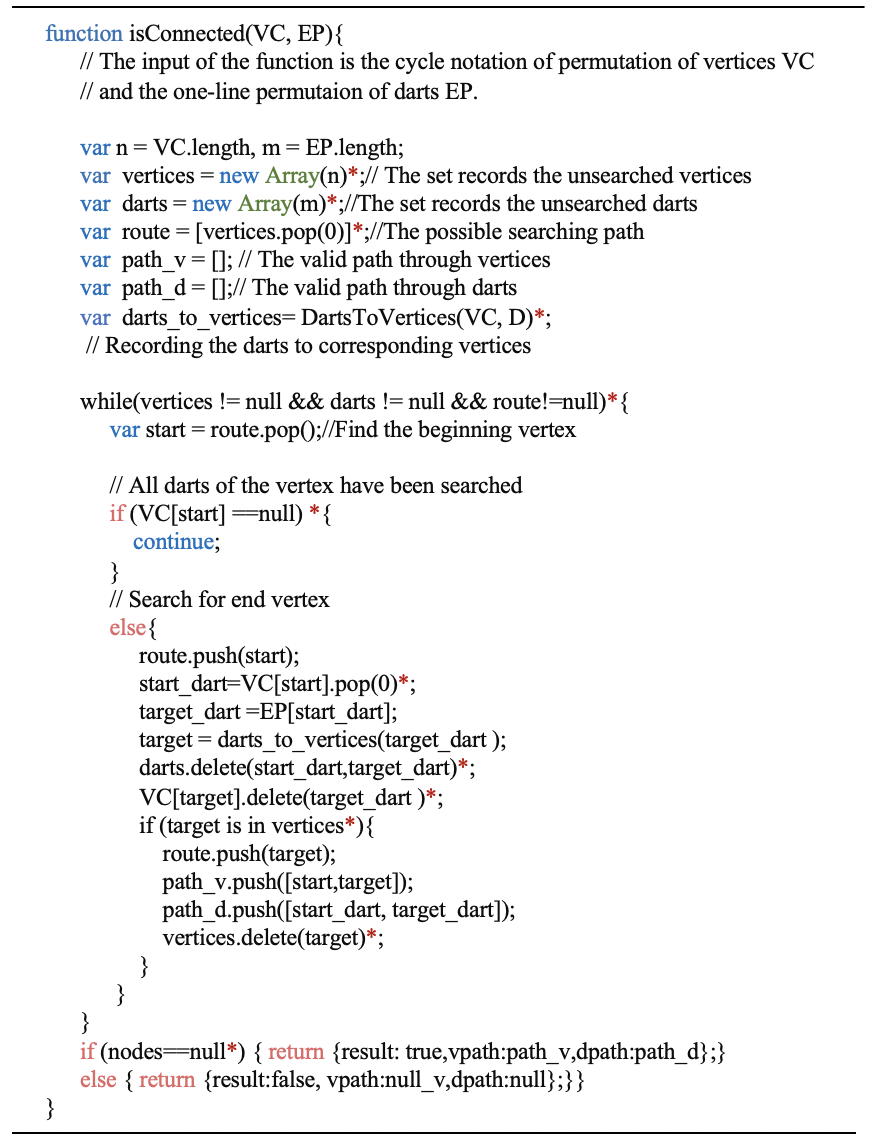
\includegraphics[width=1\textwidth]{../../image/DFS.png}
    \caption{The rough implementation of DFS by JAVASCRIPT, the lines with \textcolor[RGB]{176,35,24}{*} are not the standard JAVASCRIPT code.}
    \label{fig:figures:DFS}
  \end{figure}

\newpage
\subsubsection{Tree drawing algorithm}
Recent paper by Christoph Buchheim et al \cite{buchheim2002improving} introducing a method for drawing a n-ary trees with \(O(n)\) time complexity. It is an improvement of the method for drawing binary trees proved by Edward Reingold and John Tilford \cite{reingold1981tidier}. Bill Mill’s article \cite{milldrawing} described the evolution of the algorithm. There are six principles should be considered when draw a tree:
\begin{itemize}
    \item[a)] The edges cannot be cross with each other.
    \item[b)] The nodes in the same depth should be kept in the same height.
    \item[c)] The whole tree should be as narrow as possible.
    \item[d)] The vertical position of parent nodes is the middle of their children.
    \item[e)] Wherever the subtree lies in a tree, it should move the same distance with its parents.
    \item[f)] For the n-ary tree, the children should divide the space evenly for their parents. 
  \end{itemize}

  For obeying the first four principles, the algorithm searches the tree from bottom to up for settle the nodes, namely, post-order traversal of the tree. When maintain the fourth principle, the parent nodes move to right and the right child of it should move toward right also, which leads to a bad result that right children in a node will cover the left children of the later nodes, in another word, some of the nodes will be disappeared. The principle e) aims to solve the problem. In order to achieve the principle, the concepts of mod, contours and threads had been proposed. The mod records the distance that the current tree should be moved, and then, moving each tree with the accumulated mod value from its ancestors to itself. This concept can solve the problem mentioned above, but it cost the running time as it needs two times to search the tree. The contours and threads make the algorithm less complexity, which looks each subtree as a block.The contour is the leftmost side of trees (minimum x-coordinate) called \textit{left contours} or the rightmost side of trees(maximum x-coordinate) called \textit{right contours} as the example in the \cref{fig:figures:subtree}. The threads are the link in the contours if the two nodes have no relationship.

  \begin{figure}[htb]
    \centering
    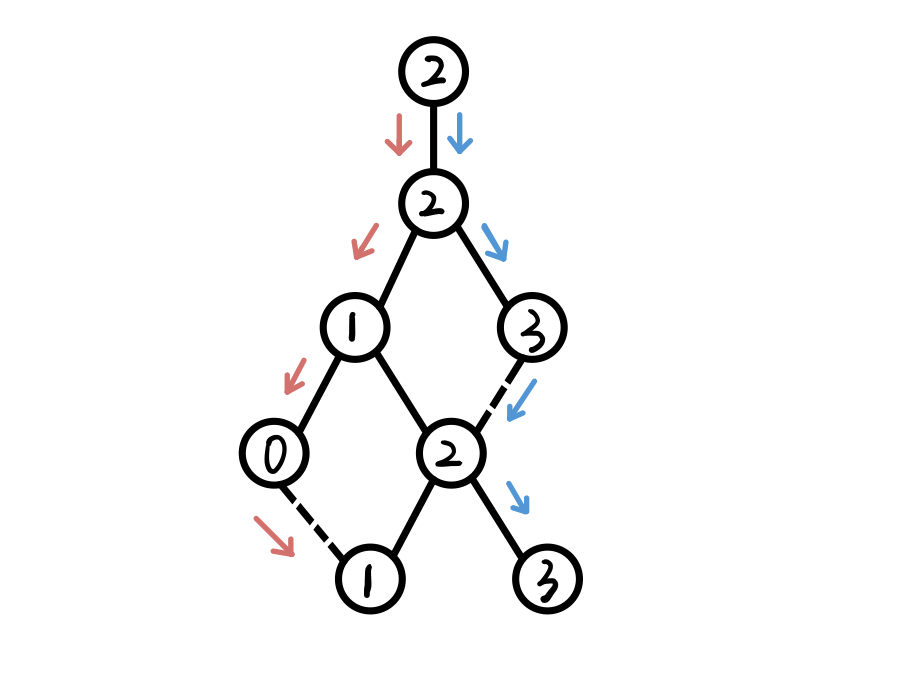
\includegraphics[width=0.8\textwidth]{../../image/subtree.png}
    \caption{The red lines show the left contour [2,2,1,0,1], and blue lines are right contour [2,2,3,2,3]. The dash lines are the threads.}
    \label{fig:figures:subtree}
  \end{figure}
  \newpage
  The thread can reduce the complexity and avoid the conflict between the subtrees, which helps to calculate accumulated mod value during the first walk of the tree. The last principle is specifically set for the n-ary tree. Since each parent might has more than two children, the left contour and right contour cannot totally deal with the conflict the problem. The concept of the ancestor is used to decide which left siblings conflicts with current subtree.

  \begin{figure}[htb]
    \centering
    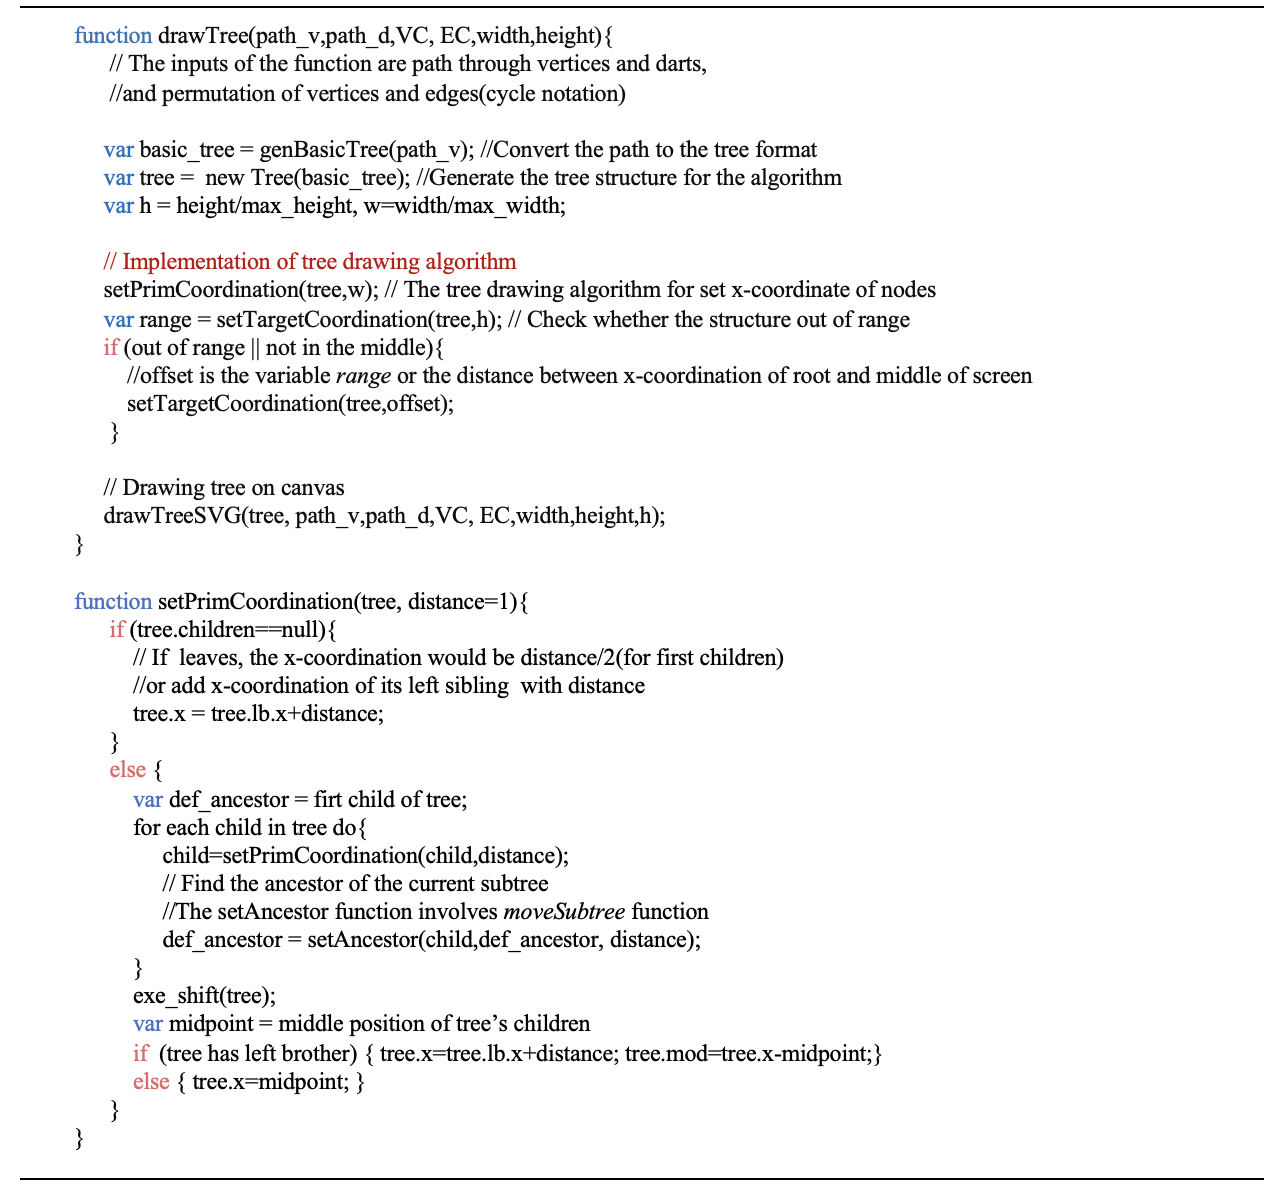
\includegraphics[width=1\textwidth]{../../image/drawtree.png}
    \caption{The constructor of tree drawing function and tree drawing algorithm in the JAVASCRIPT implementation.}
    \label{fig:figures:drawtree}
  \end{figure}

  \newpage
  The tree drawing algorithm just concerns on how to calculate the x-coordination, rather than fill the structure into a certain canvas. It is necessary that computing the vertical and horizon gap between each nodes. The horizon gap can be calculate directly, just using height of canvas divided by max depth of the tree. The vertical gap can be conducted by the same way, while, it is more difficult to compute the max width for the tree. The weighted average method is used to solve the problem. Firstly, generating a list \textit{wide} which records the width for each level of trees. Sorted \textit{wide} with ascending order as the next step. Finally, the weight of each item in \textit{wide} is the serial number of the item divided by the length of \textit{wide}, and the computing the weighted average of items. 

  The function \textit{drawTreeSVG()} in \cref{fig:figures:drawtree} is to do the drawing work on the canvas with D3.js. The coordination of the nodes and the path of links should be collected as a list, after that, drawing the model in a specific area. The \cref{fig:figures:treedraw} shows the result of the implementation of tree drawing algorithm.

  \begin{figure}[htb]
    \centering
    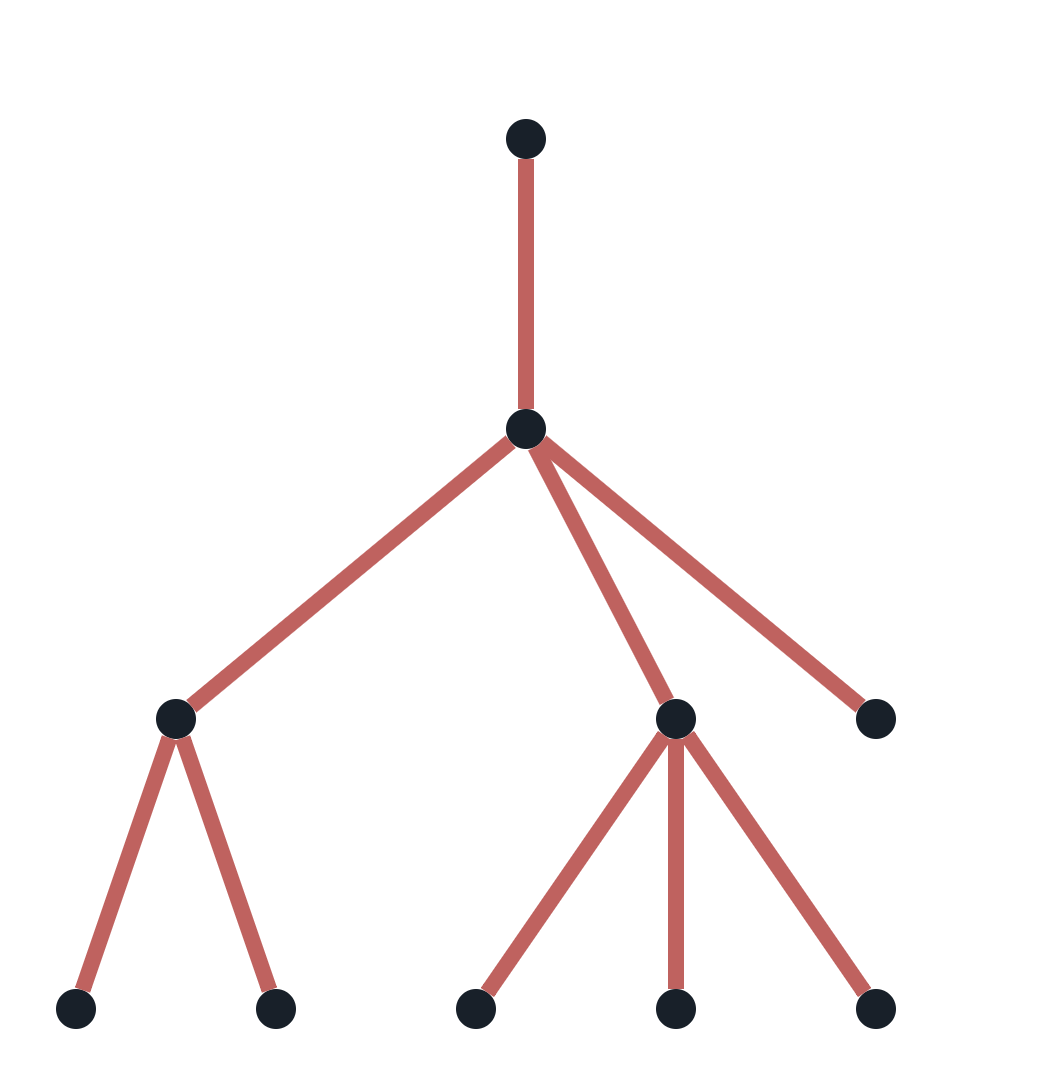
\includegraphics[width=0.6\textwidth]{../../image/treedraw.png}
    \caption{Result of the algorithm.}
    \label{fig:figures:treedraw}
  \end{figure}
  \newpage
  We have already got the tree sketch of the combinatorial maps. Some of darts are fixed within the tree structure, while the rest should be settled according to the existed darts. It uses the same approach to calculate the coordination of the endpoints of remaining darts in \textit{vertices based method}. 

  \begin{itemize}
    \item[a)] Find two darts around the same vertices.
    \item[b)] If there is no darts between them, return a).
    \item[c)] Otherwise, calculate the angle between them using \(angle=atan2(v1.y,v1.x)-atan2(v2.y,v2.x)\) ( and \(angle=angle+2*\pi\) , if \(angle<0\)).
    \item[d)] \(N\) is the number of darts between them, and the radian \(rad\) between each nodes is the \(angle/(N+1)\). The less valued darts is seen as the base line, and \(v1\) is the direction vector for base line.
    \item[e)] For \(n=1 \, to\, N\), \(d_n.x=v1.x*cos(rad*n)+v1.y*sin(rad*n)+v.x\) and \(d_n.y=-v1.x*sin(rad*n)+v1.y*cos(rad*n)+v.y\) where \(v\) is the vertex which the darts surrounding.
    \item[f)] Repeat the above steps until all the darts are placed. 
    \item[g)] Connect the new darts rely on the permutation of edges.
  \end{itemize}

  \subsubsection{Bezier curves} 
  For the purpose of  receiving a sleek and smooth edge, the connection using curve line rather the straight. Bezier curve is an algorithm to calculate a curve between to endpoints. Unlike other splines, the Bezier curve must through the start and target points. The degree of curvature depends on the control point. Second-order Bezier curve has one control point and third-order Bezier curve has two.  In this method, the third-order Bezier curve is being used. The control points are the extending along the direction of corresponding darts.

  \begin{figure}[htb]
    \centering
    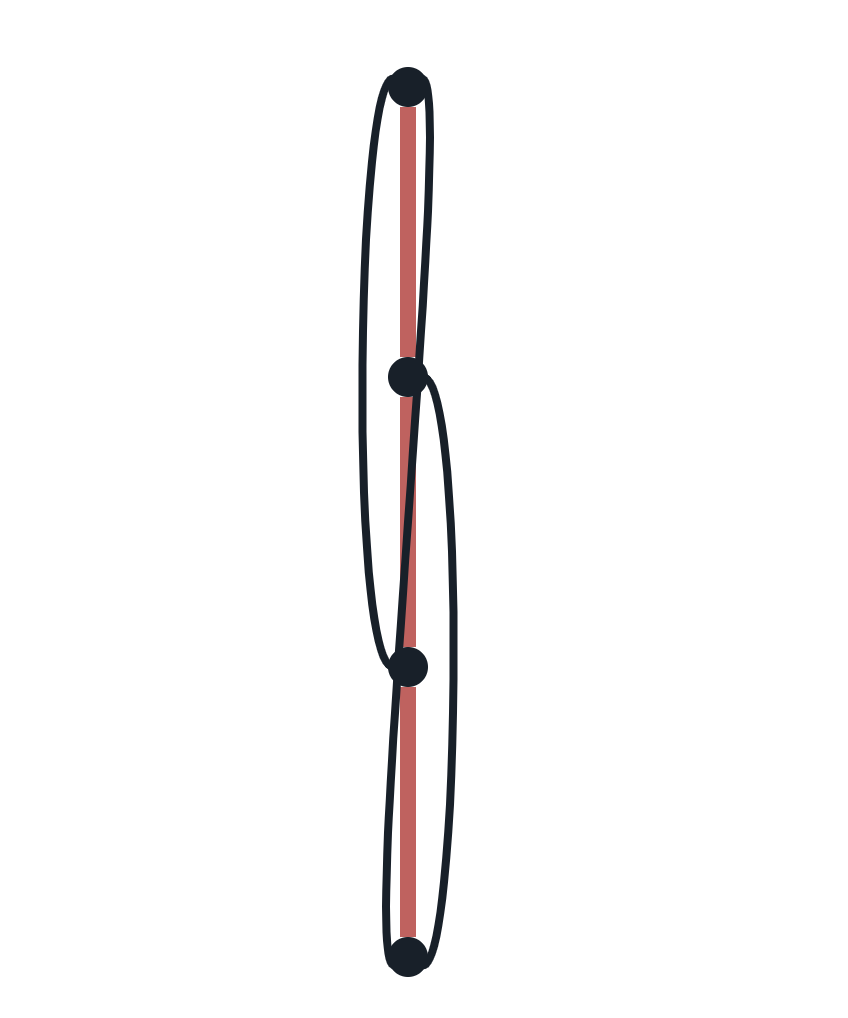
\includegraphics[width=0.5\textwidth]{../../image/example1.png}
    \caption{Result of the method for visualisation of the combinatorial map about Planar Tetrahedron(planar map).}
    \label{fig:figures:example1}
  \end{figure}

  \subsubsection{Problem}
  The result in \cref{fig:figures:example1} is a planar maps. It has been mentioned that the planar maps is a cross-free model, while in the \cref{fig:figures:example1}, the crossing occurs. As the same time, for the Petersen graph in the \cref{fig:figures:pertersengraph1} has 2 genus, which means that it is not necessary to avoid the cross as much as possible. 

  \begin{figure}[htb]
    \centering
    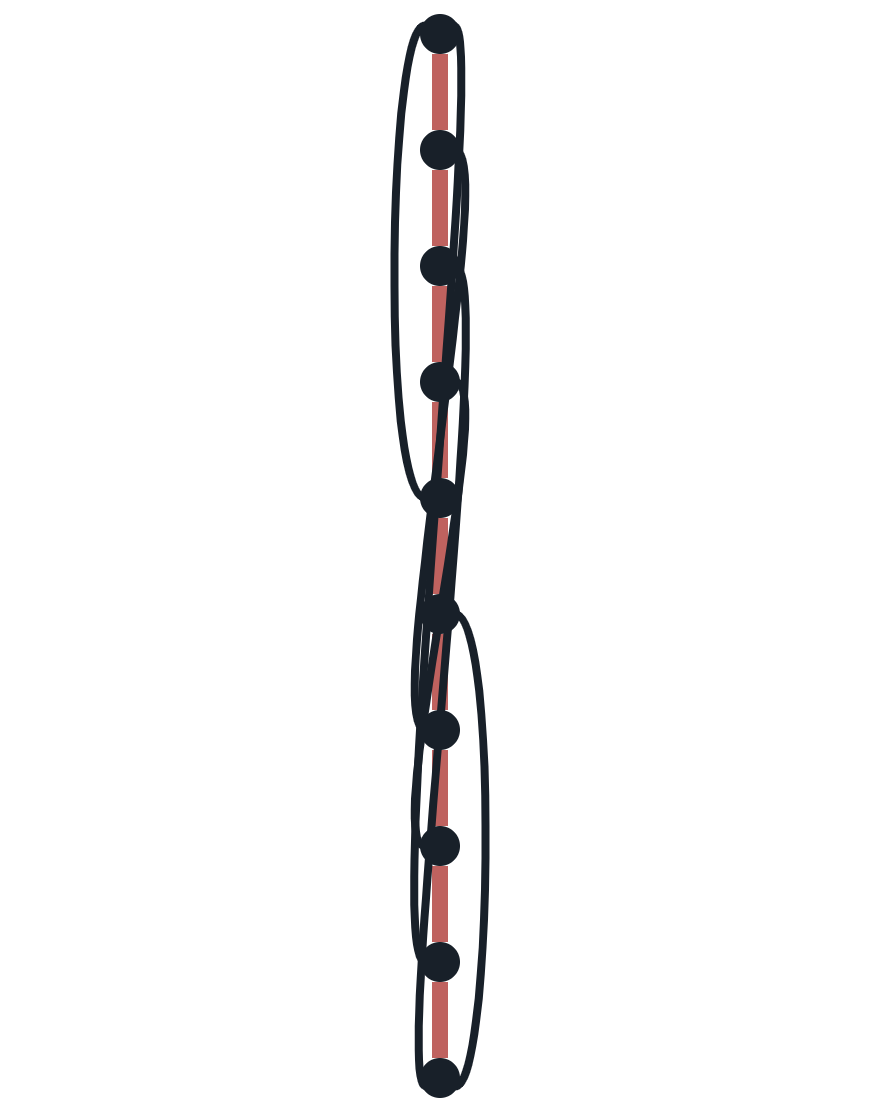
\includegraphics[width=0.4\textwidth]{../../image/pertersengraph1.png}
    \caption{Result of the method for visualisation of the combinatorial map about Petersen graph.}
    \label{fig:figures:pertersengraph1}
  \end{figure}

  However, the edges look so mass and entangled that every edges cannot be read directly. The traditional way is label the corresponding number in the end of each half-edges but this makes the image more disordered and unclear. The tips and highlight are added to indicate each vertices and edges like \cref{fig:figures:highlight}.

  \begin{figure}[htb]
    \centering
    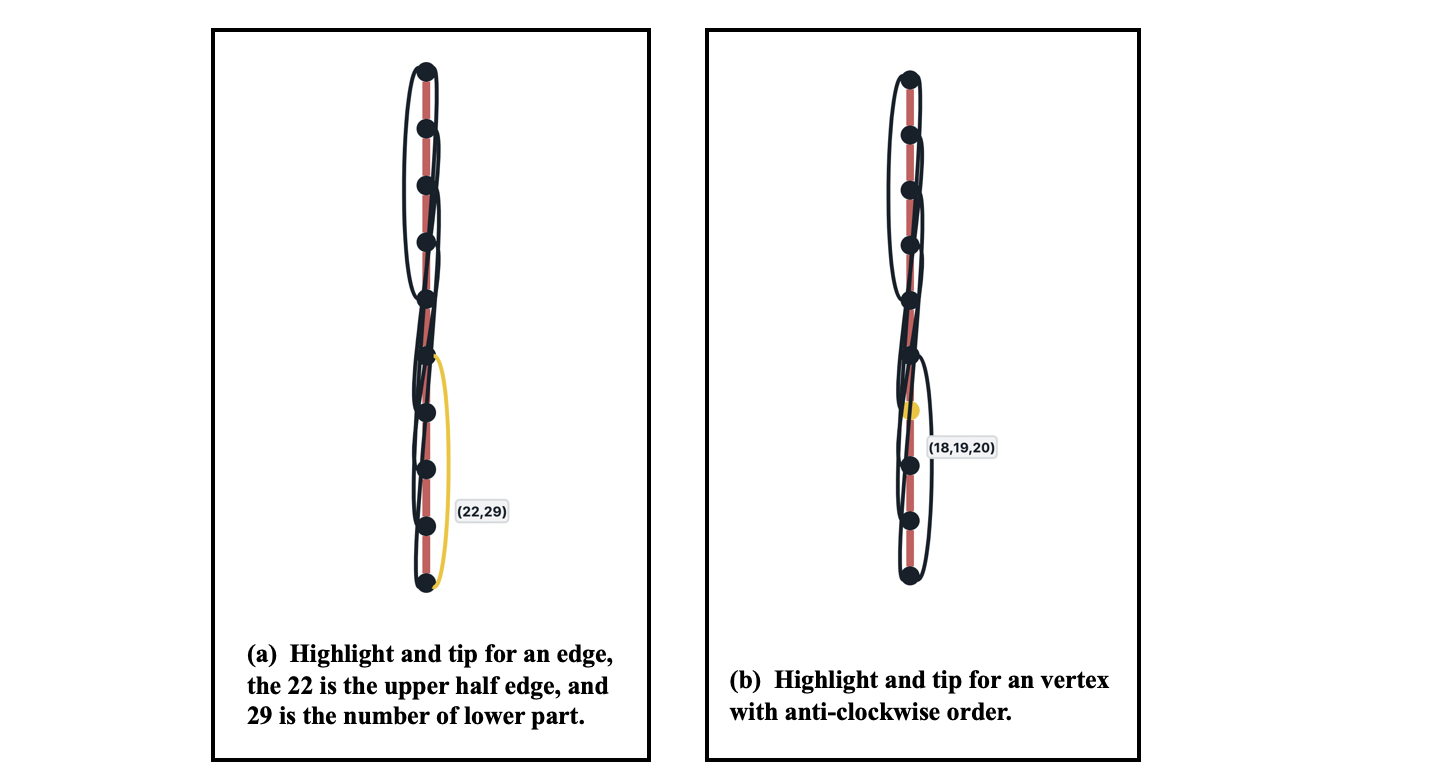
\includegraphics[width=0.8\textwidth]{../../image/highlight.png}
    \caption{The tips and highlights example.}
    \label{fig:figures:highlight}
  \end{figure}

  \subsubsection{Improve version}
  The main issue about hardly avoiding the cross for planar map is the position or direction of darts around a vertex. The spanning trees (as the result of DFS algorithm) of most combinatorial maps are a straight line, like the red part in the examples. When settle the extra darts , in the previous method, it is just divide the angles between excited darts. This leads to absolutely opposite directions for a two darts which should be connected. Therefore, the result of the connection using Bezier curve will through the middle line rather than cross the line.

  On behalf of improving the darts angle problem, an idea is to involve the darts as virtual nodes into the tree structure. That is to say, each vertex has darts essentially and it might also have children in the spanning tree structure, so as to drawing the darts as the virtual children for a vertex in the tree structure. After that, one or some of the darts are connect to the other darts who are belongs to the children vertices of the current one in the original tree model. The \cref{fig:figures:improbvetree} shows the transformation. The circles filled white are types of virtual nodes, one is the joint of two darts in the tree structure, and another one is the darts of the vertices.

  \begin{figure}[htb]
    \centering
    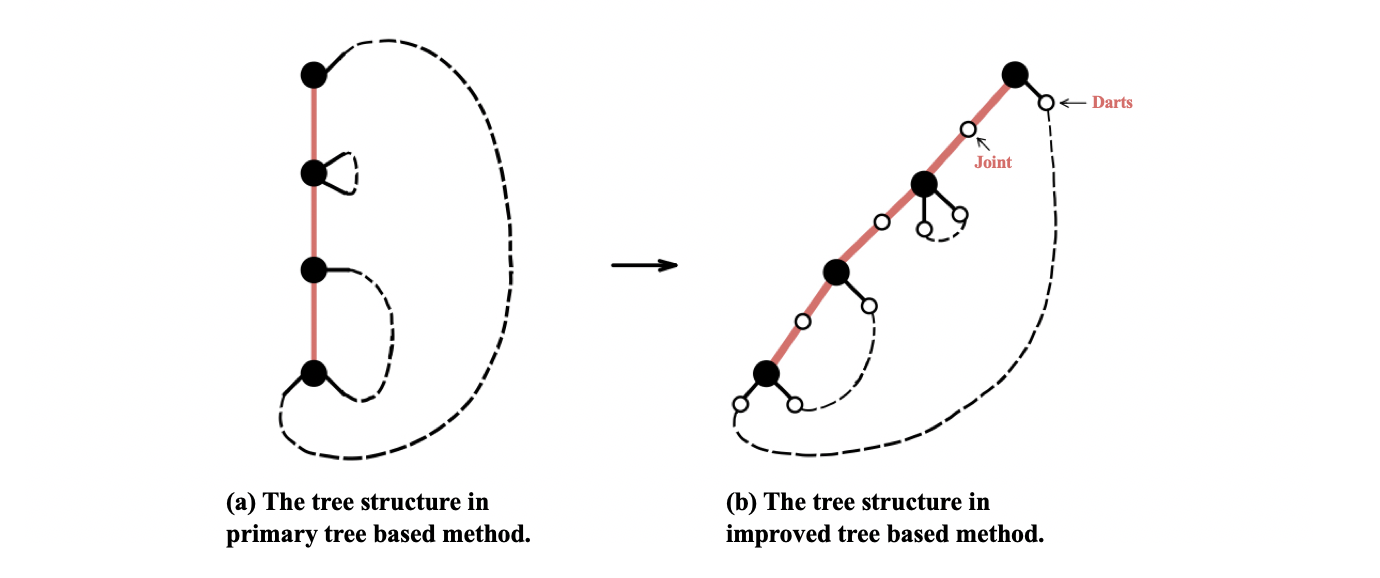
\includegraphics[width=0.8\textwidth]{../../image/improbvetree.png}
    \caption{The compare between tree structures in two methods.}
    \label{fig:figures:improbvetree}
  \end{figure}

  Redefining the tree structure is not enough to avoid the cross, some situation of the connection have to discuss too. (Note: Reverse direction of a dart in all situations means doing the mirror inversion according to the \(x=x_d\) where \(x_d\) is the x-coordination of the dart.)

  \begin{itemize}
    \item[a)] If the less x-coordination node towards left and larger one to the right, the curve should through the bottom.
    \item[b)] The extension of two darts are cross. This station still arrives the bottom but the direction of both are reversed.
    \item[c)] If any of the two darts is the middle children of its father, the direction of the middle dart is horizon.  This connection also go via bottom.
    \item[d)] The last situation is both darts are toward the same direction. For the right side, if the less y-coordination node has larger x-coordination, reverse the lower node and connect them through the bottom, otherwise, the connecting line will go through the middle node of two darts. It is the same for the right side.
    \item[e)] Last but not least, counting the numbers of connections through bottom, left and right, respectively. Using corresponding lines to divide the each space. All are using 3-order Bezier curves.
  \end{itemize}

  \begin{figure}[htb]
    \centering
    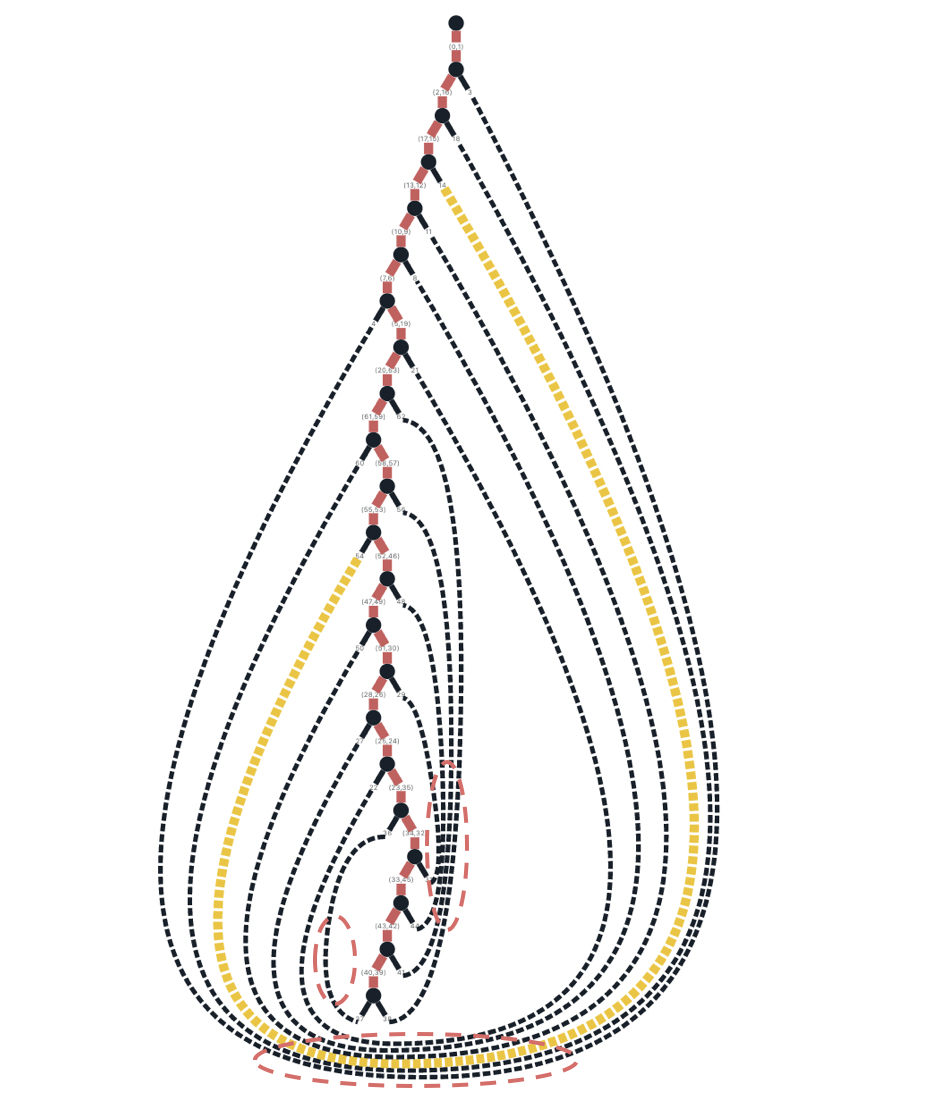
\includegraphics[width=0.6\textwidth]{../../image/improvemap.png}
    \caption{The result of improved tree based method for rooted dodecahedron graph.}
    \label{fig:figures:improvemap}
  \end{figure}

  This method has greatly reducing the cross, and the oval with dash line demonstrate the essence of the ideas. As the mean time, it do not need extra time to calculate the position of darts which out of the tree structure. Due to dividing the fix size of the area, the gap between lines are narrow. Highlight the selected line can produce a simple and convenient recognition of it.

  \subsection{Face Based algorithm}
  This approach comes from the dual of map. If it succeed, it might recover the surfaces which the  combinatorial maps embedded in.

  \subsubsection{Dual}
  Any embedded graph has its dual graph in the same surface. The vertices of the dual structure is the centre of the corresponding faces in the combinatorial map. The darts around the vertices in the dual map are the darts surrounding the primary faces.

  \begin{figure}[htb]
    \centering
    
\includegraphics[width=1\textwidth]{../../image/dual.png}
    \caption{The dual map of  a combinatorial map.}
    \label{fig:figures:dual}
  \end{figure}

  The core of the idea which comes from this structure is generating every faces of the combinatorial maps. Gluing the faces together by connecting the corresponding darts under the edges permutation. With the help of folding algorithm, the drawing results are improving from 2-dimensional to 3-dimensional which shows the underlying surfaces that the maps embedded in.

  \subsubsection{Visualisation}
  The fundamental task is to drawing the faces without gluing. It is necessary that separating the screen into \(N_f\) parts where \(N_f\) is the number of faces. Firstly, judging whether the \(N_f\) can be squared. If possible, the result is denoted as \(n_l\), and the screen splits into \(n_l\) rows and \(n_l\) columns. If it is not , dividing the canvas into 3 lines and \(abs(N_f/3)+1\) columns. The next step is drawing each faces, it is easy to find that each face is a polygon, bilateral(with two vertices) or loop(with one vertex).

  \begin{figure}[htb]
    \centering
    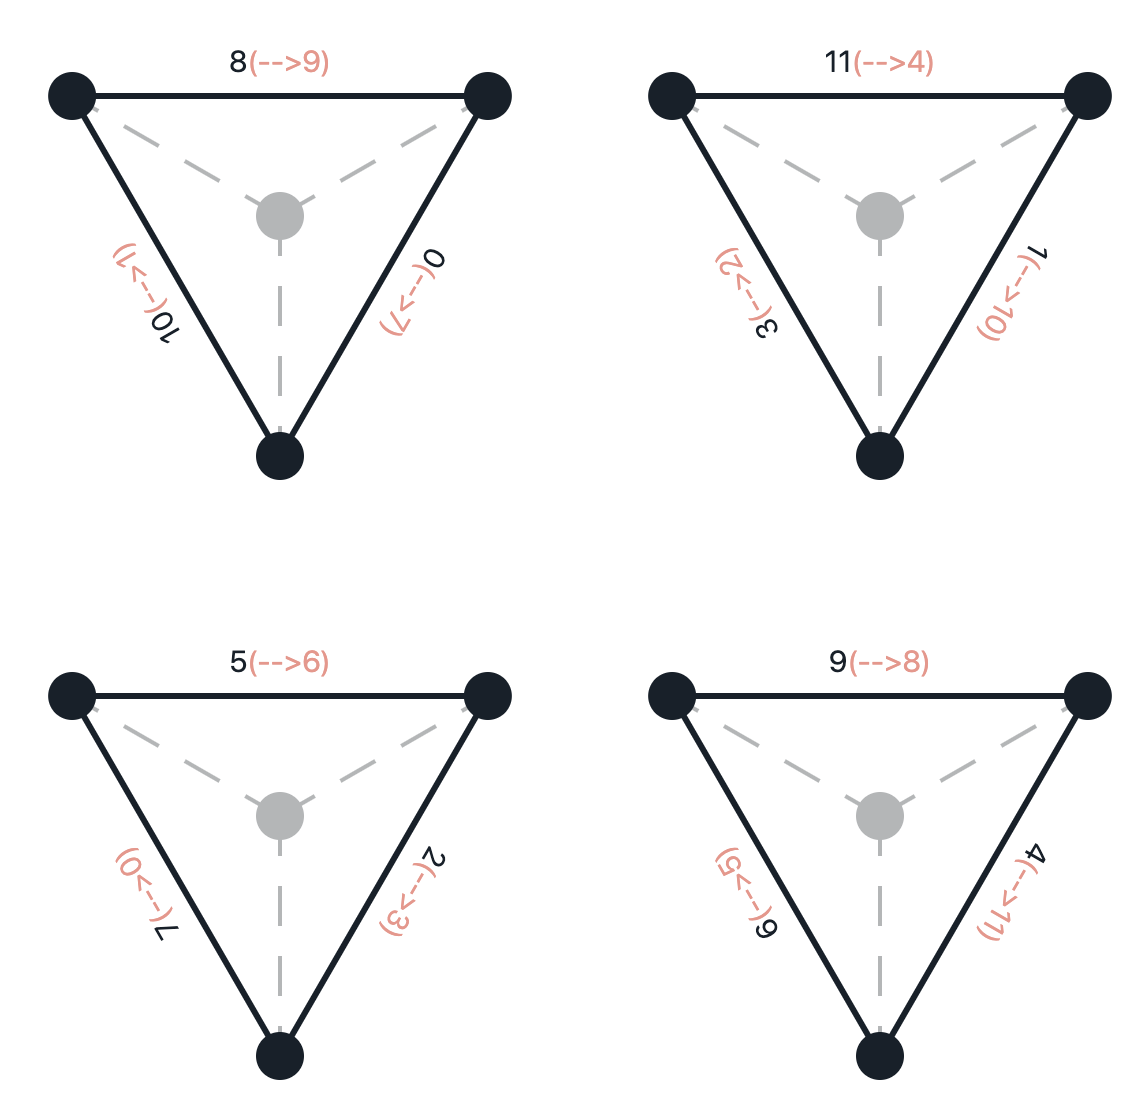
\includegraphics[width=0.5\textwidth]{../../image/facesmap.png}
    \caption{The visualising of a combinatorial map for planar tetrahedron by faces based method.}
    \label{fig:figures:facesmap}
  \end{figure}

  The labels of the darts are the darts number (black words) and the red numbers indicate which darts to connect with. The grey nodes and dash lines are the corresponding parts in dual maps.

  \section{Tool Structure}

  A tool aims to package the methods for visualisation of combinatorial maps as a website application. This section covers the structure of the tool including two pages: introduction and visualiser, as well as introducing how does each section work. The style for the layout of pages uses Bootstrap.css \cite{bootstrap2019}, and the icon in the pages also from the bootstrap opening icon set \cite{openicon2019}.

  \subsection{Introduction}
  The purposes of the tool are not only displaying the combinatorial maps, but also helping the researchers or beginners reward the knowledge of it. Therefore, an introduction page is necessary to deliver the basic background of maps, the features which the visualiser involved, and the other informations for example what algorithm are implemented. This is also seen as the starting page.

  \subsubsection{Head}
  The head of the page is to describe why the tool should be created and provide the links. The right button ‘Get start’ goes to the visualiser page if people want to experience the tool directly, while the left one stays at the local page to let people learn more about the theory knowledge.
  
  \begin{figure}[htb]
    \centering
    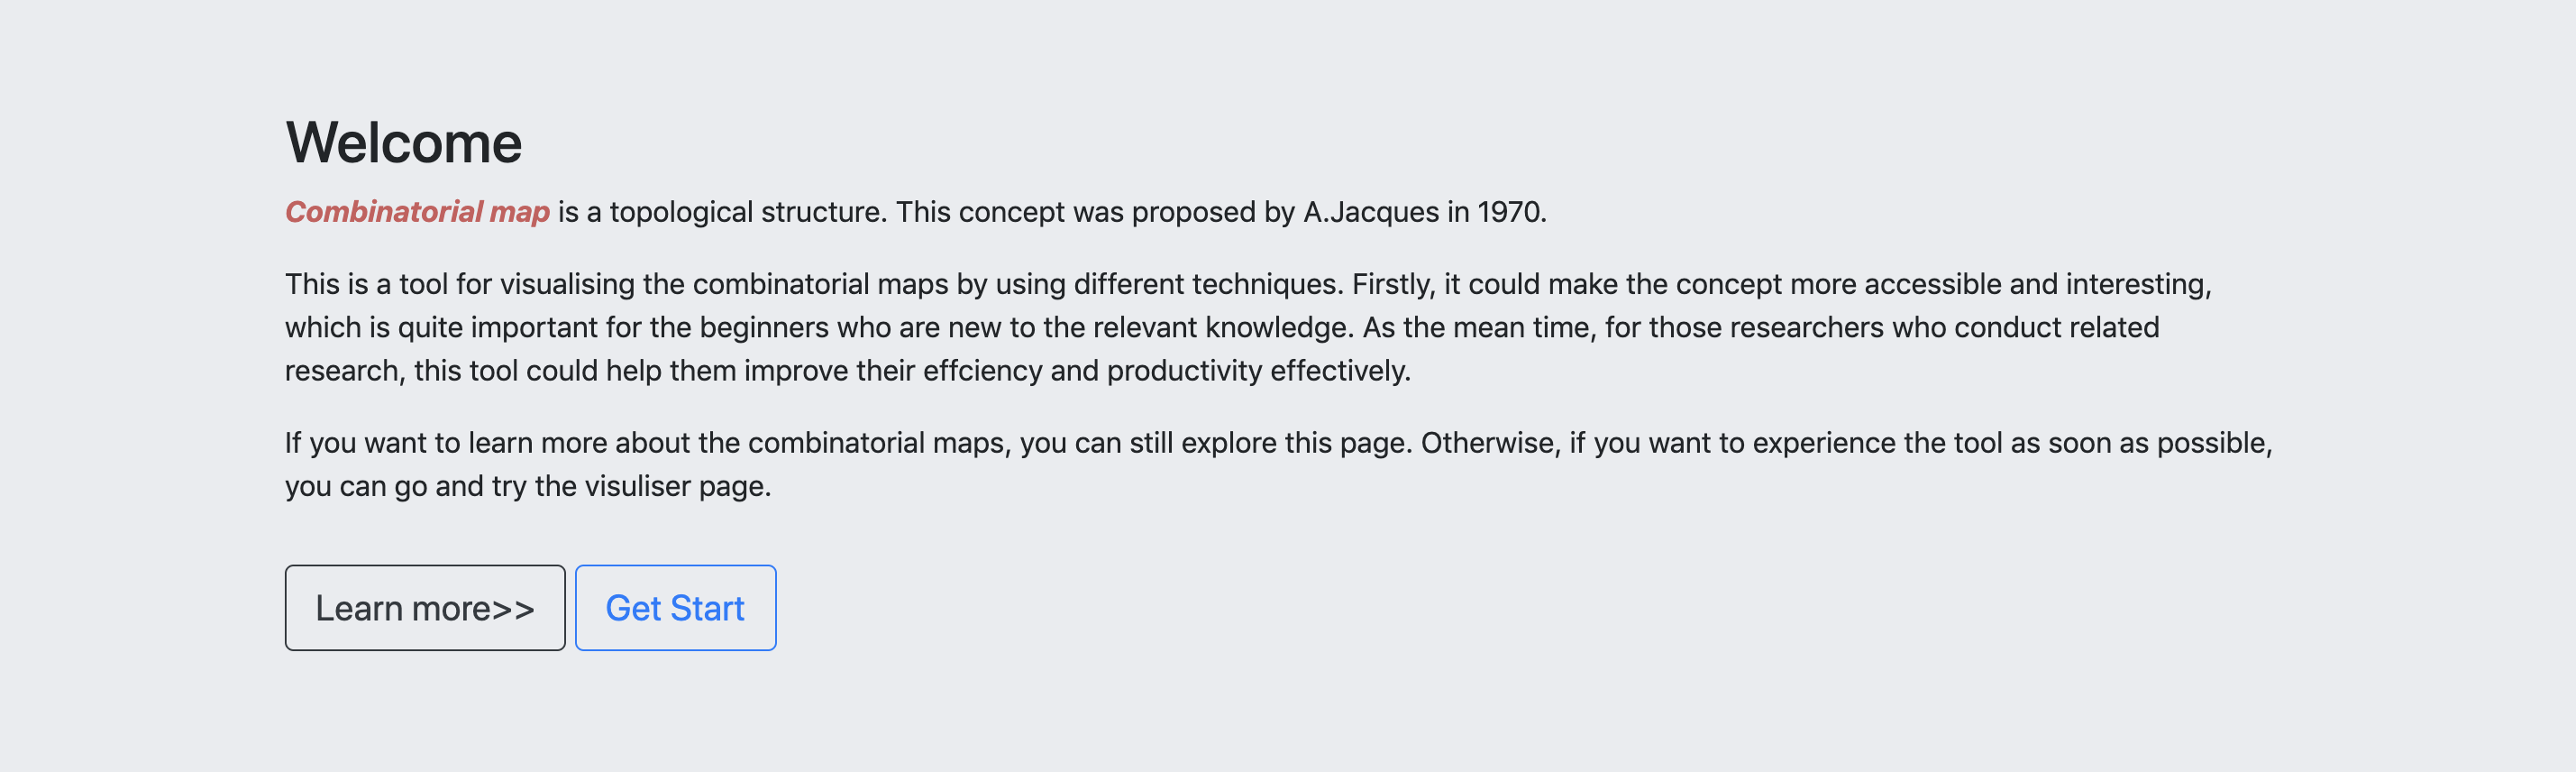
\includegraphics[width=1\textwidth]{../../image/head.png}
    \caption{The head of the introduction page.}
    \label{fig:figures:head}
  \end{figure}

  \subsubsection{Main content}
  The side bar of the main content is a table of content plugin \cite{tocplugin2019}. From the guideline of the content,  we can see that the there are three sections about combinatorial maps, visualiser and relevant algorithms. If people want to know more informations, just click the item and it will link to the specific area in the page. It can jump to the visualiser to another page when click icon beside the subtitle named visualiser.
  
  \begin{figure}[htb]
    \centering
    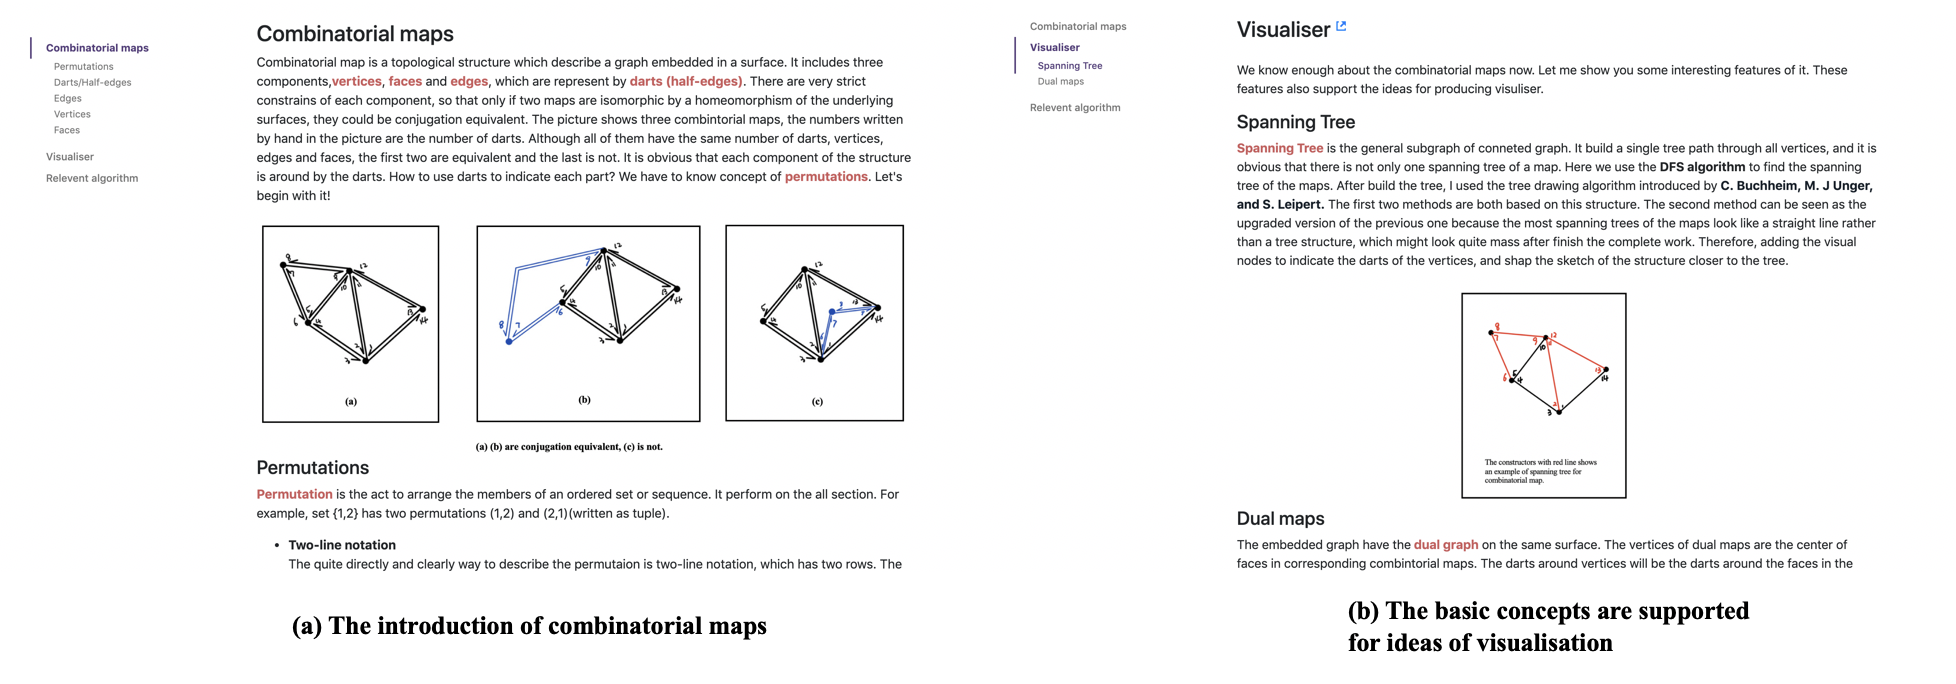
\includegraphics[width=1\textwidth]{../../image/content.png}
    \caption{The content of the introduction page.}
    \label{fig:figures:content}
  \end{figure}

  \subsection{Visualiser}
  This page plays an essential role in the whole project. It is divided into three parts, the introduction, input and output. 

  \subsubsection{Introduction}
  The page has the introduction part, as well. The introduction can help the users have a clear mind about the structure of page and know the operations and limitation of each parts. The button `learn more' means return to the introduction page to learn the knowledges of combinatorial maps and the tool. The `get start' is starting to try the visualiser.
  
  \begin{figure}[htb]
    \centering
    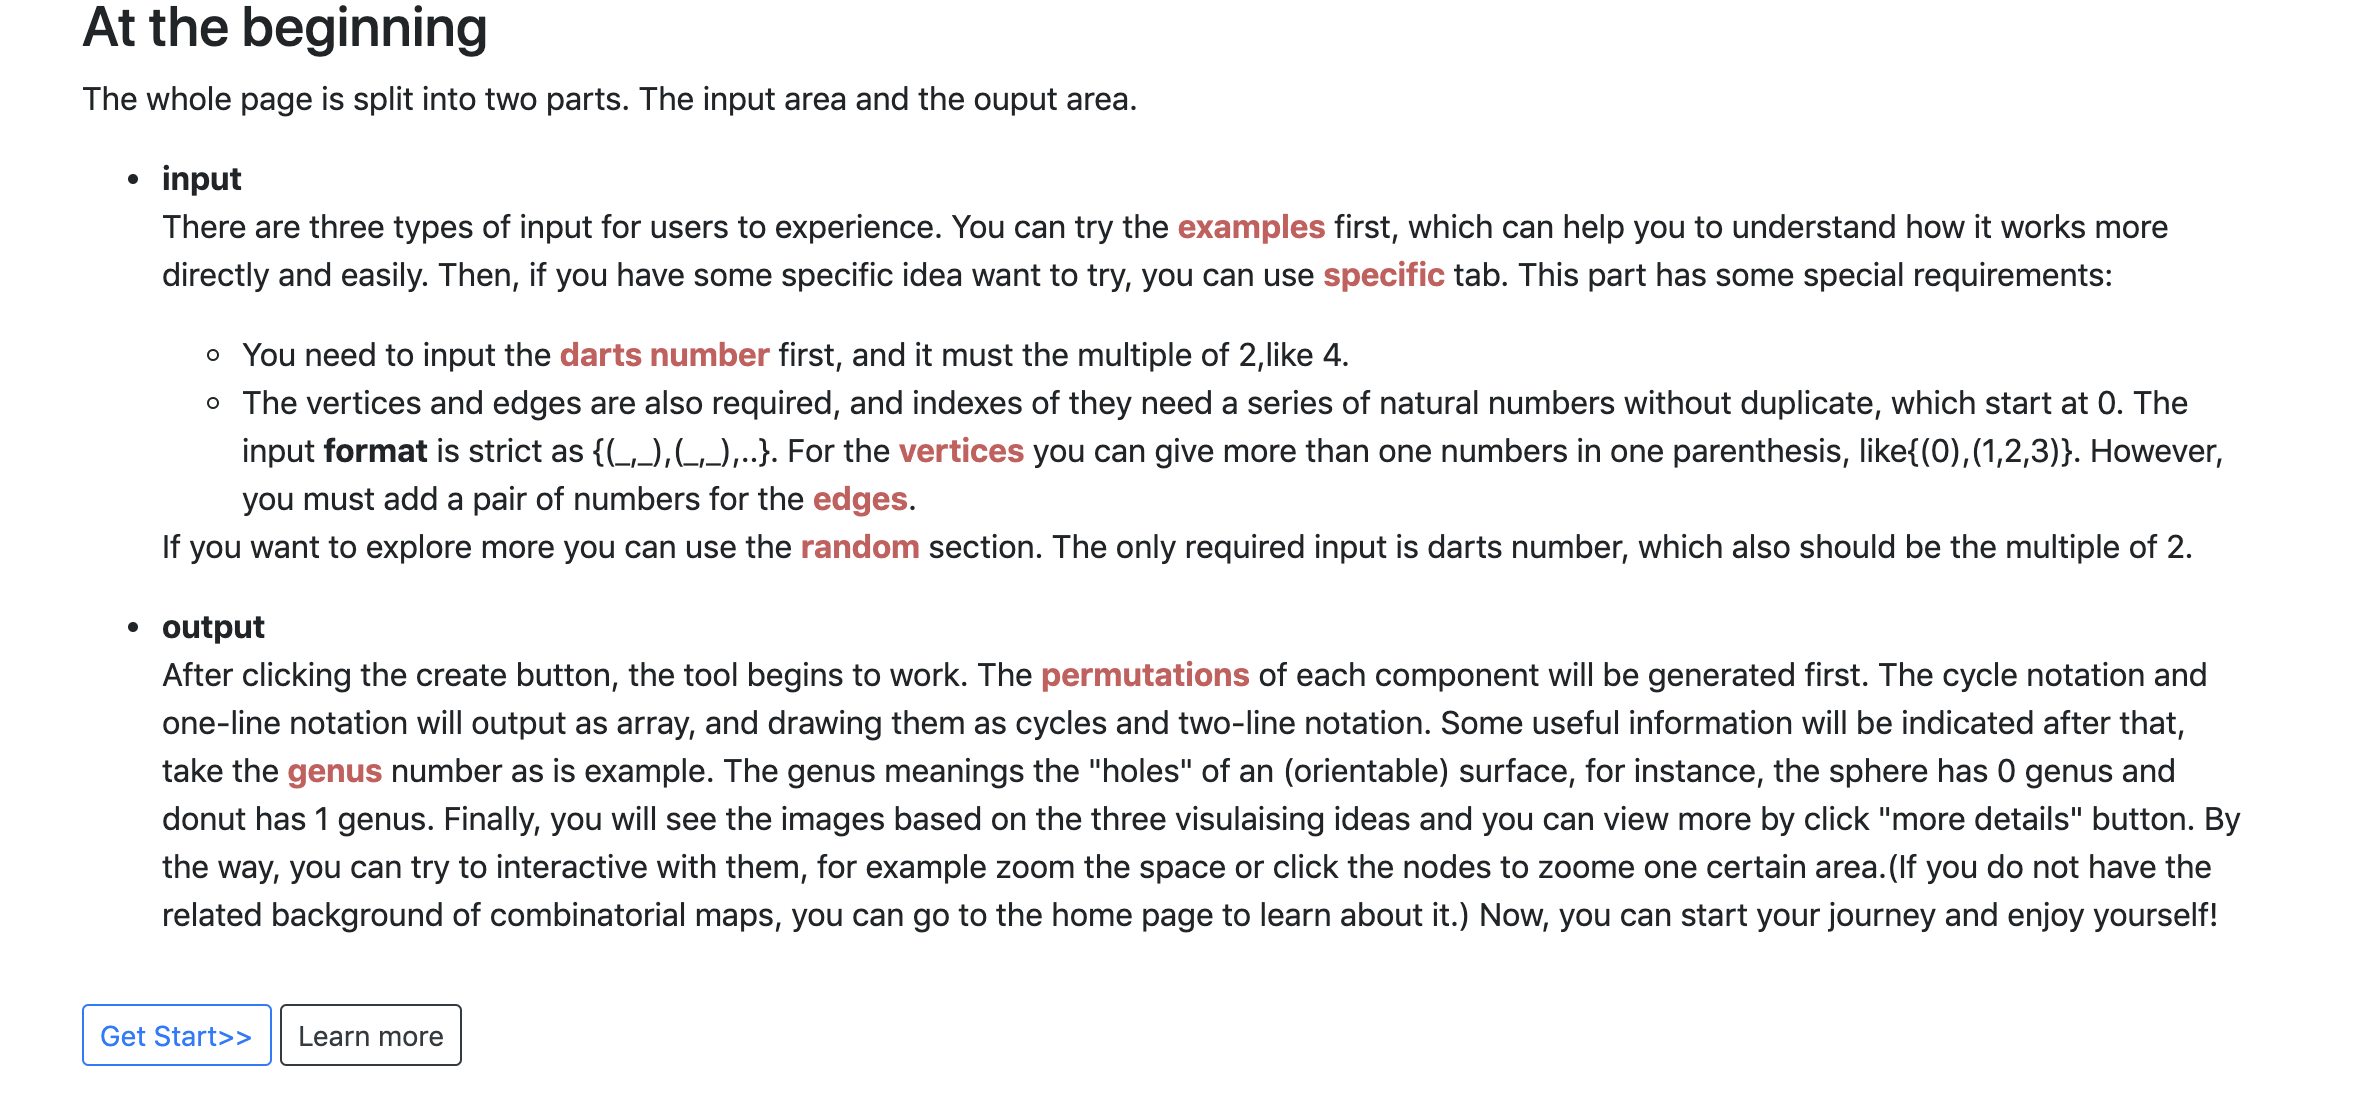
\includegraphics[width=1\textwidth]{../../image/head2.png}
    \caption{The introduction of visualiser page.}
    \label{fig:figures:head2}
  \end{figure}

  \subsubsection{Input}
  There are three type of input methods for users to choose, examples, specific and random.

  \begin{itemize}
    \item[a)] Users can select an arbitrary example as input to experience how tools work. All the examples are classical combinatorial maps including planar and non-planar maps. Click the `create’ button, the tool start to do the visualisation.
    \begin{figure}[htb]
        \centering
        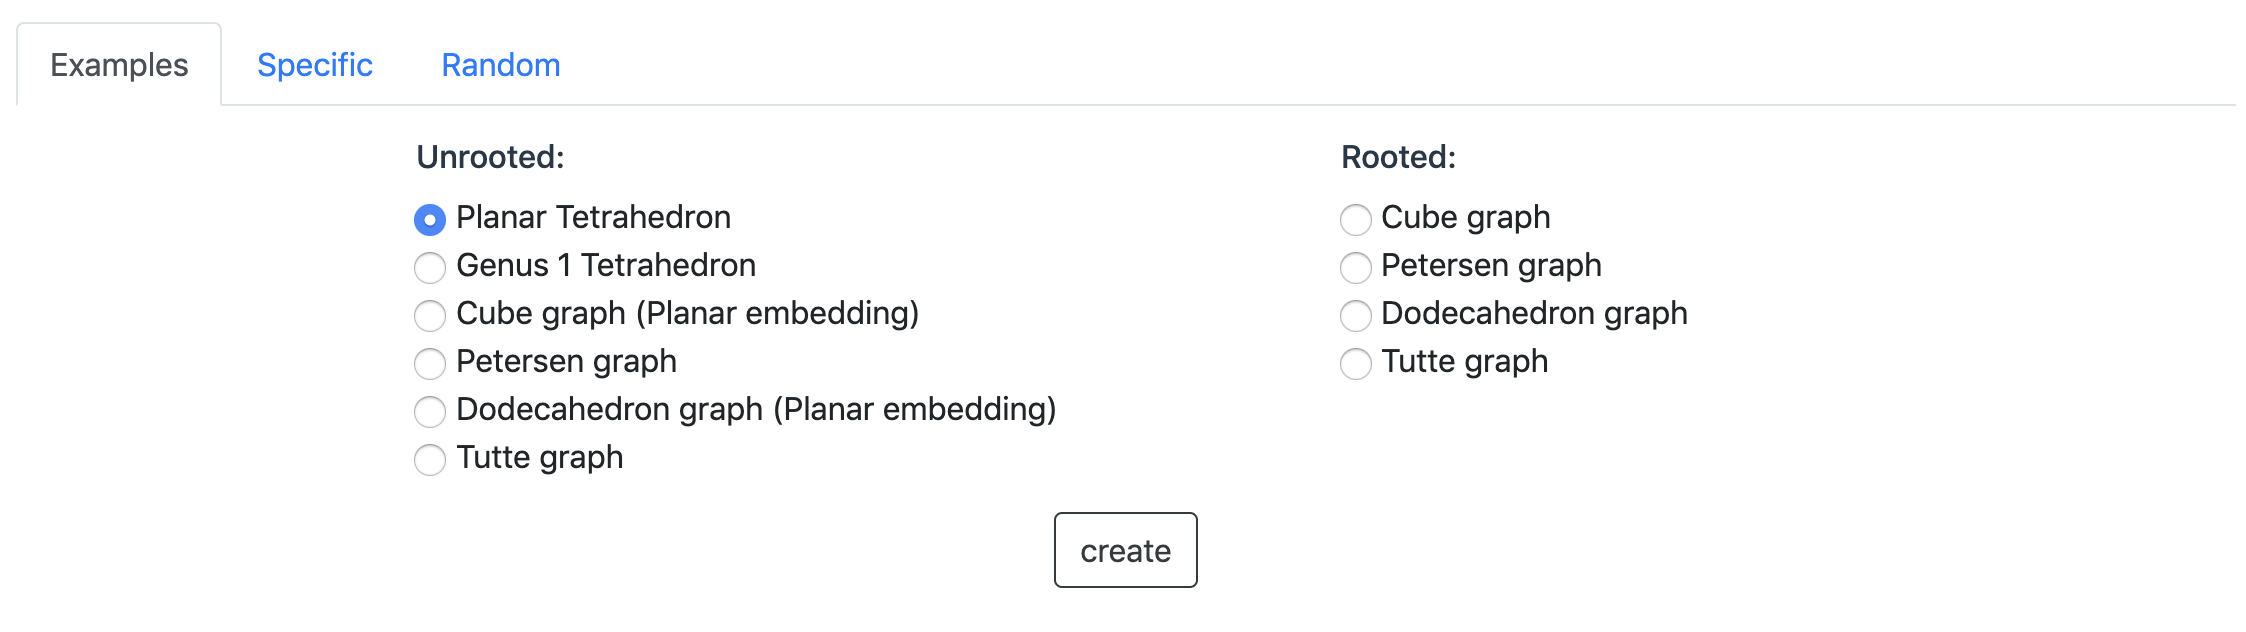
\includegraphics[width=1\textwidth]{../../image/exampletab.png}
        \caption{The examples tab}
        \label{fig:figures:exampletab}
      \end{figure}
    \newpage
    \item[b)] If users have a certain sample which is not included in the given examples, he or she can choose the  ‘specific’ tab. Three pieces of information are required, the darts number and the permutation of vertices and edges with cycle notation. The darts number should be filled at first and correct,otherwise, users cannot continue doing other operations.
    \begin{figure}[htb]
        \centering
        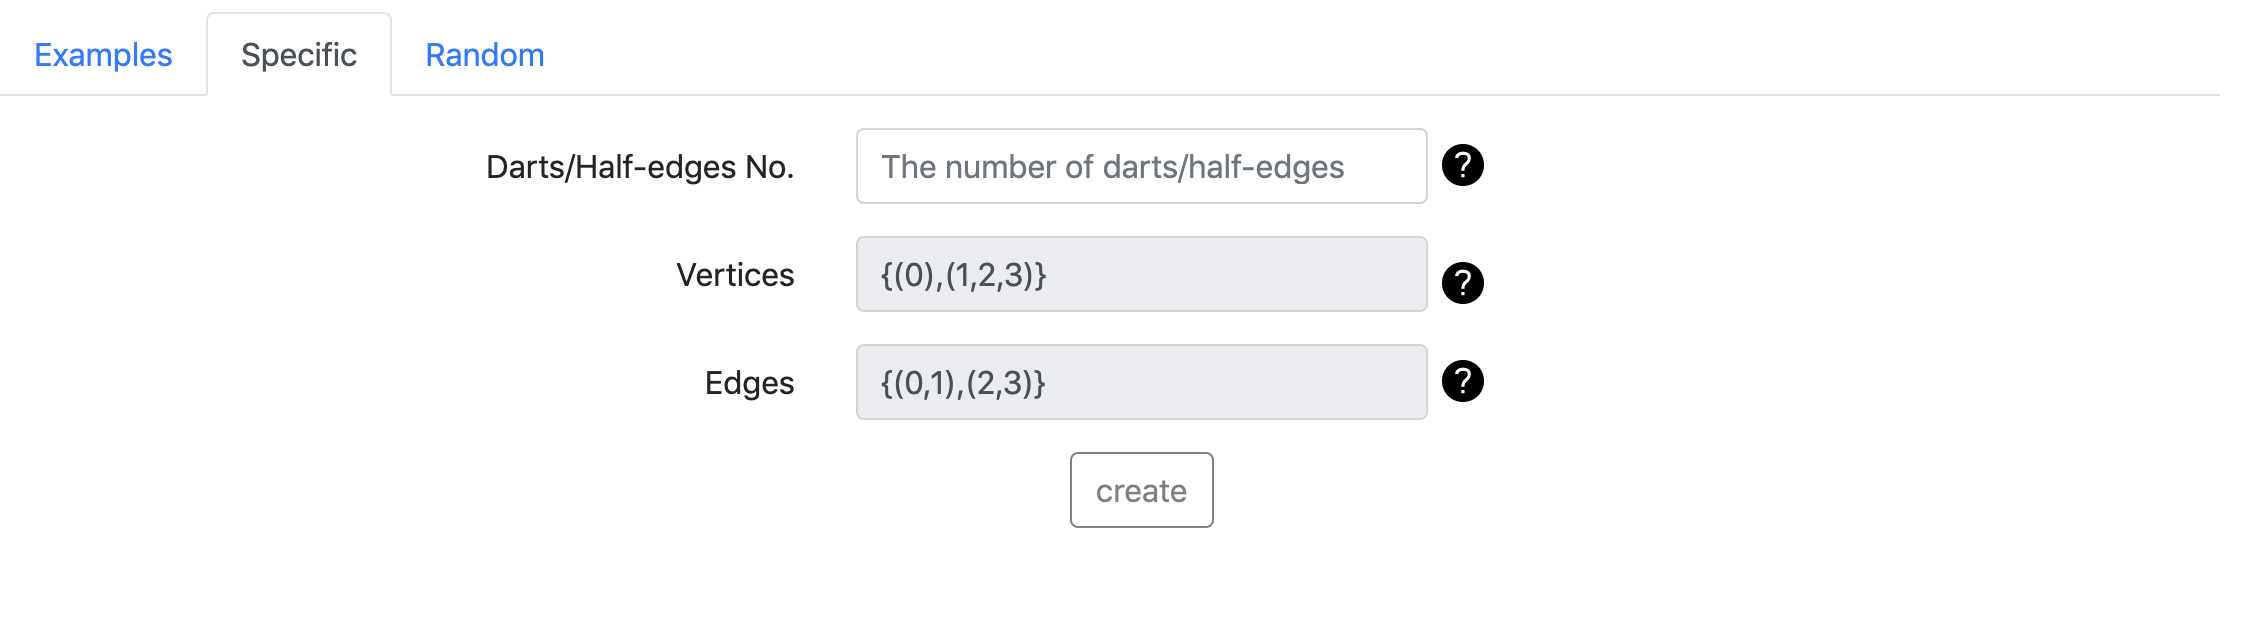
\includegraphics[width=1\textwidth]{../../image/specifictab.png}
        \caption{The specific tab}
        \label{fig:figures:specifictab}
      \end{figure}

    Some conditions are used to validate whether the input is correct or not. A JAVASCRIPT library called Vue.js\cite{you2018vue} is used to do the real-time validation and data communication.  Firstly, for the darts number, it must be a number that is multiple of 2. Secondly, the permutation of vertices and edges have their own format the users should obey, for example, the numbers of each permutation must be a series of natural number start from 0 and the largest number must be the darts number minus 1. For the vertices, the numbers of elements in the parentheses must more than 1, while, in edges permutation, it can only have two numbers. These constraints provide a structural clue to parse the inputs whose data type is string. For parsing the string to a readable and operational data type, a regular expression is used, for instances, the expression ‘/\^{}\textbackslash\{(\textbackslash([0-9]+(,[0-9]+)\textbackslash))(,\textbackslash([0-9]+(,[0-9]+)\textbackslash))*\}\$/’ matches the format of inputted edges. The real-time validation will check the input at every time when users change the content. If the wrong input, the system will promote the users with an error massage and provide a right examples. The users can also click the `?’ button to check the requirement of the inputs.
    \begin{figure}[htb]
        \centering
        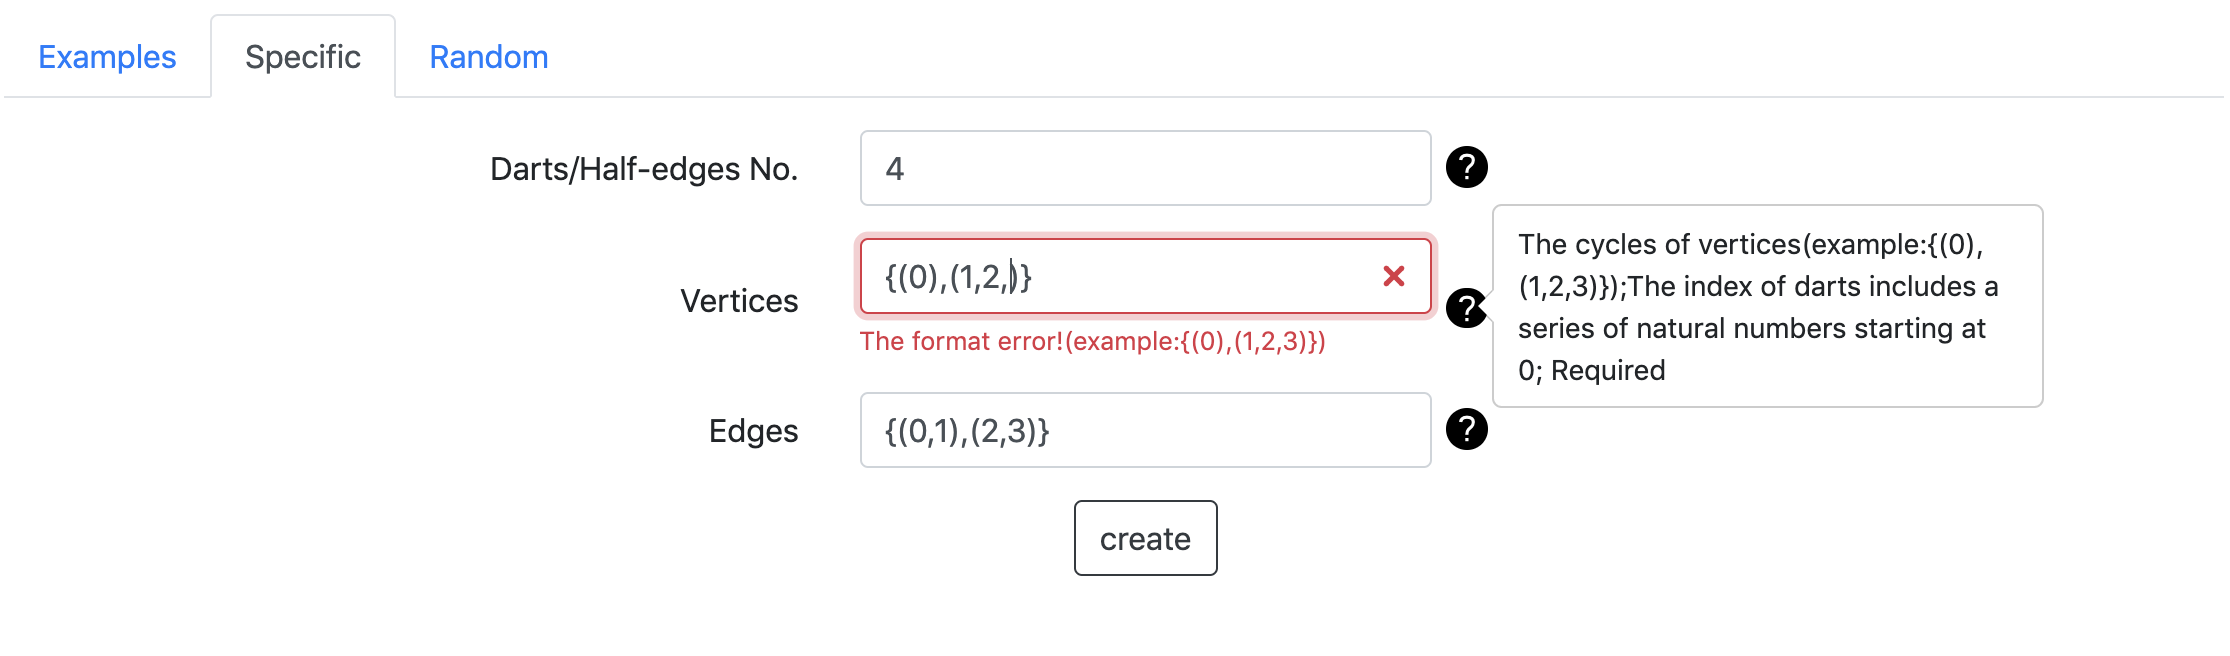
\includegraphics[width=1\textwidth]{../../image/errorinput.png}
        \caption{The error massage and notes.}
        \label{fig:figures:errorinput}
      \end{figure}
    
    \newpage
    \item[c)] The last tab is for users who do not have a specific example of combinatorial maps or those who just want to seek various results of maps with the same darts number, hence the darts number is required. Meanwhile, users can decide whether needs to limit the number of vertices for the map and the number must not more than darts number.
    \begin{figure}[htb]
        \centering
        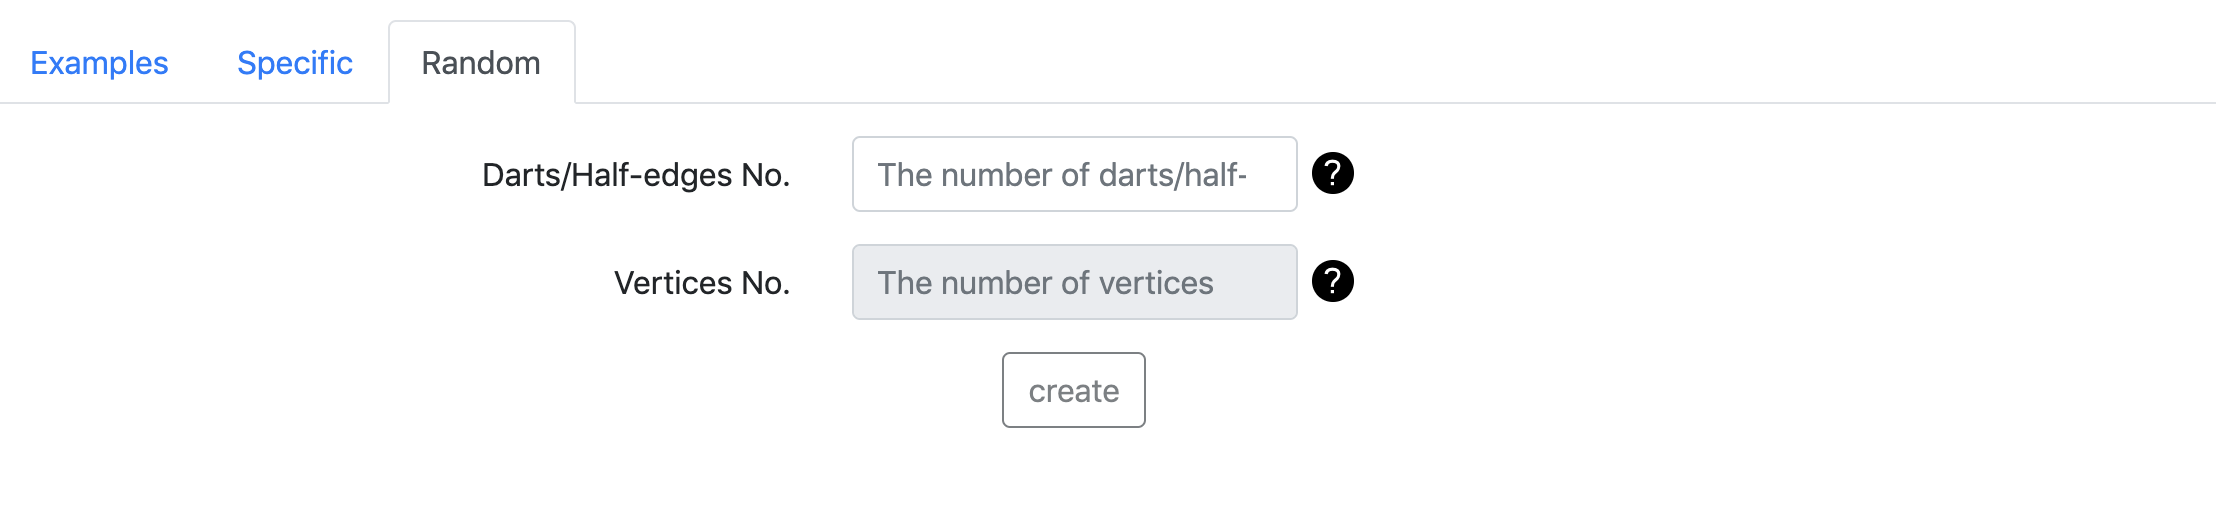
\includegraphics[width=1\textwidth]{../../image/randomtab.png}
        \caption{The random tab}
        \label{fig:figures:randomtab}
      \end{figure} 
      
    Regardless of whether the user has entered the number of vertices, the entire process starts with generating a random permutation of edges \textit{genRandomEdges()}: 1.Defining a set of darts \(D\); 2. Choosing arbitrary two members of it and delete them; 3. Pushing selections as array into the edges array \(EC\); 4.Repeating 2 and 3 steps until \(D\) is empty. 

    Creating the permutation of vertices is the next step, which depends on whether the users enter the number of vertices. If the input is empty, using Fisher-Yates shuffle algorithm \cite{fisher1943statistical} to generate a vertices permutation with one-line notation \textit{genRandomVerticesPerm()}. The logic of the function is as below: 1. Declaring a set \(VP\) whose length is the number of darts \(n_d\) and the elements follow the natural order; 2.For each member whose index is \(i\), selecting a random number \(j\) from 0 to \(n_d -1\); 3. Swapping the elements \(VP[i]\) and \(VP[j]\). 
    
    Another function \textit{genRandomVerticesByNum()} is used when the input is not empty as \(n_c\).  At the beginning, defining a set \(VC\) which has \(n_c\) members of empty array. The core of the function is a loop with period \(n_d\). For each time \(n\), randomly choosing a number \(r_d\) between 0 and \(n_c -1\). Adding \(n\) to the array \(VC[r_d]\). Redefining \(VC\) if any of the element is still empty. Actually the random function the JAVASCRIPT defined is useless and unfair, thus, a new random generator is defined. Even though, it still need to verify that whether the \(VC\) contains the empty elements.

    The function \textit{convertToPermutations()} aims to convert the cycle notation to one-line notation and \textit{convertToCycles()} inverses the process. Finally, using the function \textit{isConnection()} mentioned above validates the whether the map is connected. If it is not connected, restarting from the first step or continuing to the next step when it is connected.
    \begin{figure}[htb]
        \centering
        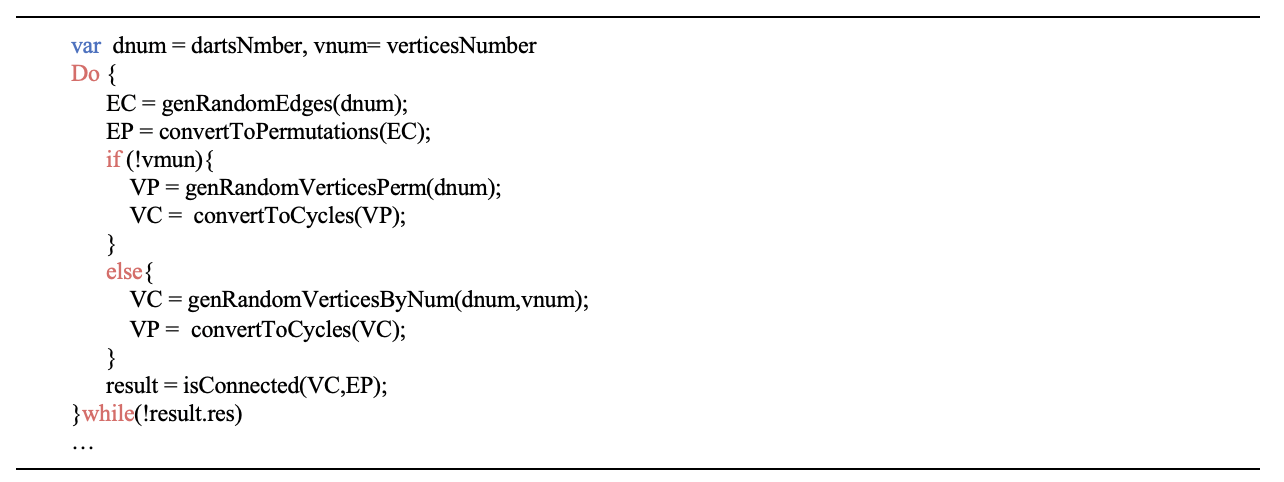
\includegraphics[width=1\textwidth]{../../image/randompro.png}
        \caption{The construct of generating a random combinatorial map with the JAVASCRIPT implementation.}
        \label{fig:figures:randompro}
      \end{figure} 
  \end{itemize}

  \subsubsection{Output}
  The output includes describing and visualising each component, displaying other information and showing the results of the approaches.
  \begin{itemize}
    \item[a)] Components of a combinatorial map. It is known that the permutation is used to indicate the permutations. In order to supporting more specific details, every notations of permutations have been visualised. The \cref{fig:figures:components} shows the results of each components, the nodes are the darts. The different colours can distinguish the components easily. It is difficult to identify the minutiae of the nodes and edges and zooming the space by click the nodes or other ways can solve the problem. The icon at the end of permutations is to reset the canvas.
    \begin{figure}[htb]
        \centering
        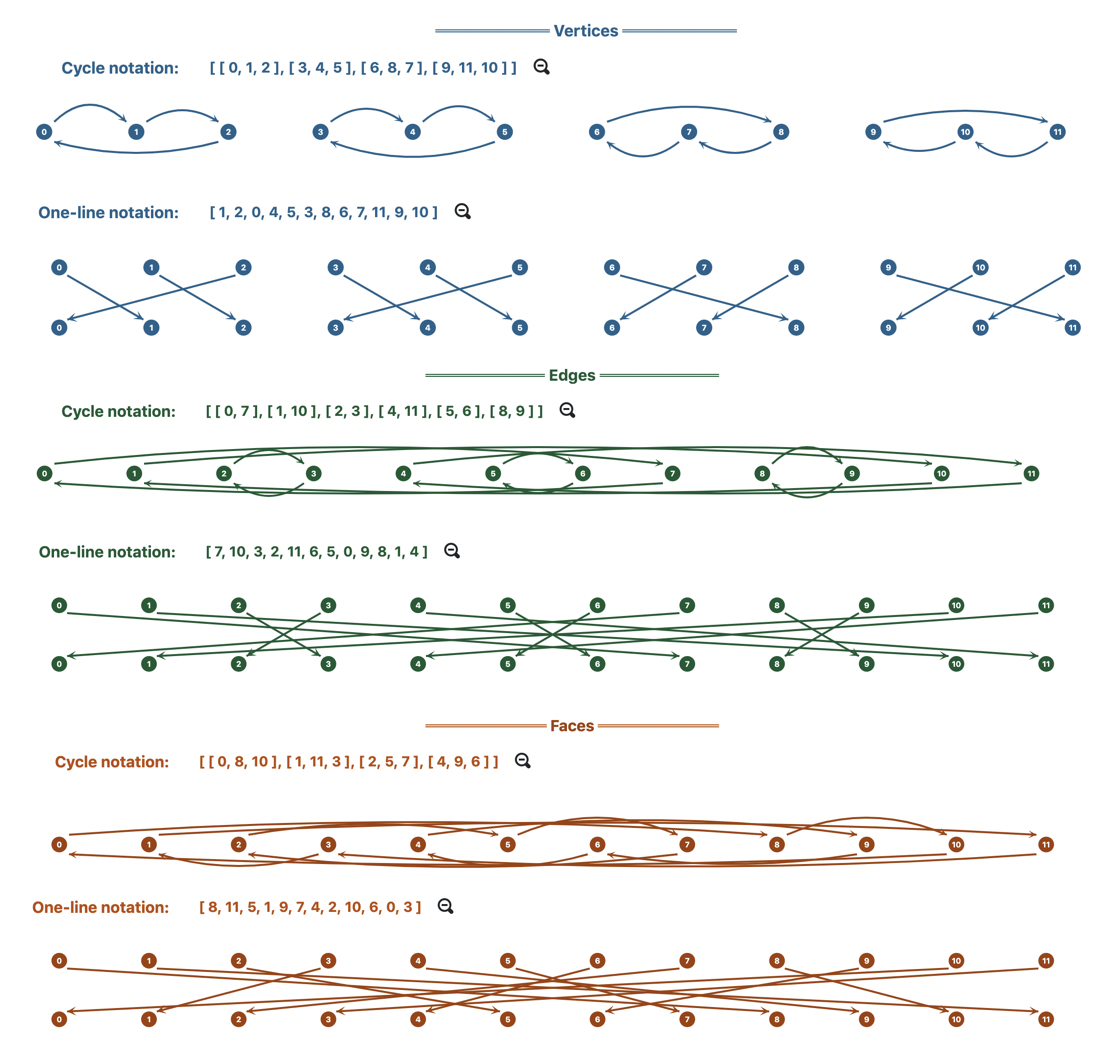
\includegraphics[width=1\textwidth]{../../image/components.png}
        \caption{Visualisation of each component}
        \label{fig:figures:components}
      \end{figure}
    \newpage
    \item[b)] Four characters faces number, vertices number, darts number and genus number are supplied in the `other characters’ area.
    \begin{figure}[htb]
        \centering
        
\includegraphics[width=1\textwidth]{../../image/otherinfor.png}
        \caption{Other information}
        \label{fig:figures:otherinfor}
      \end{figure} 
    \item[c)] The bottom of the page is the results of approaches. Every results show as PNG format, and hover effect cover on the images tell the idea of the methods. If users want to see the details, clicking the `MORE DETAILS’ button and an interface will pop out. A real SVG image displays on the interface and the necessary information is wrote at the side of it.
    \begin{figure}[htb]
        \centering
        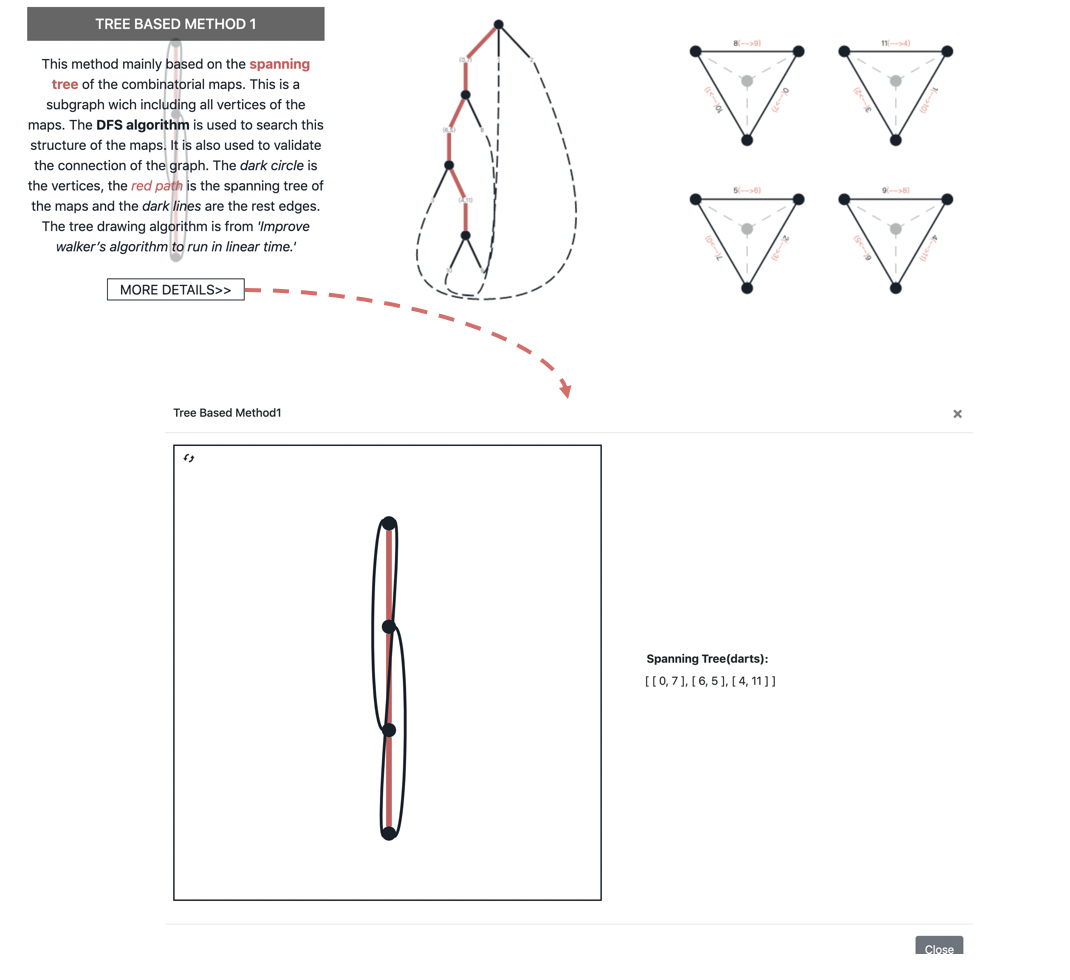
\includegraphics[width=1\textwidth]{../../image/resultsofmethod.png}
        \caption{Results of methods}
        \label{fig:figures:resultsofmethod}
      \end{figure} 
  \end{itemize}

 